\chapter{Symulacyjna weryfikacja tezy}

Weryfikacja przedstawionego w pracy modelu błędu i wynikających z niego założeń odbędzie się w pierwszej kolejności metodą symulacyjną. W bieżącym rozdziale przedstawiony zostanie przykładowy tor pomiarowy, a następnie zostaną w nim wyróżnione kolejne źródła błędów. Na podstawie przedstawionego wcześniej modelu błędu opisane zostaną związki zachodzące pomiędzy błędami i oszacowana zostanie niepewność wielkości wyjściowych analizowanego toru pomiarowego. Wyniki uzyskane za pomocą zaproponowanego modelu zostaną porównane z wynikami uzyskanymi metodą Monte-Carlo. Omawiana analiza zostanie przeprowadzona z osobna dla każdego fragmentu toru pomiarowego, a następnie na podstawie ustalonych związków między błędami oszacowana zostanie niepewność rozszerzona wielkości wyjściowych analizowanego toru pomiarowego.

Przykładowy tor pomiarowy składać się będzie z przetwornika pomiarowego, który przekształcać będzie ciągłą w czasie wielkość fizyczną $s(t)$ na reprezentujący ją sygnał napięciowy $y_{a}(t)$. Sygnał wyjściowy przetwornika pomiarowego poddawany będzie wzmocnieniu w celu dopasowania jego poziomu do zakresu napięcia wejściowego przetwornika analogowo-cyfrowego. Wzmocniony sygnał $y_{b}(t)$ podawany będzie na wejście przetwornika analogowo-cyfrowego, którego wielkości wyjściowe oznaczono symbolem $x_{c}(i)$. Ostatecznie sygnał wyjściowy przetwornika analogowo-cyfrowego trafiać będzie na wejście algorytmu dyskretnej transformacji falkowej, a na jego podstawie wyznaczany będzie wektor wielkości wyjściowych oznaczonych jako $X(k)$. Schemat ideowy opisanego toru pomiarowego przedstawiono na rysunku \ref{fig_chain_symul}.

\begin{figure}[htb!]
\begin{center}
\includegraphics{obrazki/schemat_symul}
\caption{Schemat blokowy toru pomiarowego będącego obiektem przeprowadzanego eksperymentu symulacyjnego \label{fig_chain_symul}}
\end{center}
\end{figure}

Podczas eksperymentu przyjmuje się, że przetwarzany sygnał pomiarowy będzie obarczony błędem związanym z szumem, o stałej widmowej gęstości mocy i rozkładzie normalnym. Przetwornik pomiarowy, zastosowany w celu przetworzenia analizowanego sygnału wejściowego na postać napięciową, posiadać będzie pewną częstotliwość graniczną, a jego charakterystyka nie będzie idealnie liniowa. Zastosowany wzmacniacz pomiarowy również cechować się będzie pewną częstotliwością graniczną, natomiast zakłada się, że nieliniowość jego charakterystyki będzie pomijalnie mała. Temperatura otoczenia wpływać będzie na dryf zera przetwornika pomiarowego oraz wzmacniacza, przy czym temperatura ta nie będzie mierzona, zatem jej wpływ na wyniki pomiaru nie będzie korygowany. Zastosowany przetwornik analogowo-cyfrowy wprowadzać będzie błąd związany z kwantowaniem oraz błąd związany z rozrzutem kwantów. Algorytm transformacji falkowej wprowadzać będzie do wielkości wyjściowych błąd własny związany z zaokrągleniami.

W dalszej części rozdziału omówione zostaną kolejne elementy toru pomiarowego, ich wpływ na przetwarzany sygnał oraz relacje pomiędzy błędami na wejściu i wyjściu tych fragmentów. Przedstawione zostaną również szczegółowe założenia odnośnie właściwości opisanych we wprowadzeniu fragmentów toru pomiarowego. Dla przeprowadzonego eksperymentu przyjmuje się, że przetwarzany sygnał $s(t)$ określony jest w postaci:
\begin{gather}
\dot{s}(t) = \frac{6}{10} \sin(2 \pi f_{1} t) - \frac{3}{10} \sin(10 \pi f_{1} t + \frac{\pi}{8}) + \frac{1}{10} \sin(30 \pi f_{1} t + \frac{\pi}{6}) \label{eqn_sym_in_ideal}, \\
\tilde{s}(t) = \dot{s}(t) + e_{s,r}(t) \label{eqn_sym_in_real},
\end{gather}
przy czym $f_{1} = \qty{1}{kHz}$, natomiast $\sigma_{s,r}^{2} = \frac{2}{3} \cdot 10^{-5}$. Parametry kolejnych harmonicznych przetwarzanego sygnału zostały zestawione w tabeli \ref{tab_sym_in_params_ideal}. Przetwarzany sygnał będzie próbkowany ze stałą częstotliwością $f_{s} = \qty{48}{kHz}$. Do wyznaczenia wektora wielkości wyjściowych algorytmu dyskretnej transformacji falkowej koniecznych będzie $N = 8$ próbek wielkości wejściowych tego algorytmu, na podstawie których wyznaczonych zostanie $M = 8$ próbek wielkości wyjściowych toru pomiarowego.

\begin{table}[htb!]
\begin{center}
\caption{Parametry kolejnych harmonicznych przetwarzanego sygnału niezakłóconego błędami przyjęte w przeprowadzanym eksperymencie symulacyjnym \label{tab_sym_in_params_ideal}}
\begin{tabular}[c]{| c | c | S | c |} \hline
\textbf{Lp. $i$} & \textbf{Pulsacja $\omega_{s,i}$, rad/s} & \textbf{Amplituda $E_{s,o}(\omega_{s,i})$} & \textbf{Faza $\varphi_{s,o}(\omega_{s,i})$, rad} \\ \hline
1 & $1000  \cdot 2\pi$ &  0.6 & $0$       \\ \hline
2 & $5000  \cdot 2\pi$ & -0.3 & $\pi / 8$ \\ \hline
3 & $15000 \cdot 2\pi$ &  0.1 & $\pi / 6$ \\ \hline
\end{tabular}
\end{center}
\end{table}

Eksperyment zakłada, że okres próbkowania będzie stały dla każdej próbki przetwarzanego sygnału, natomiast okno pomiarowe będzie usytuowane losowo względem przebiegu przetwarzanego sygnału. Dodatkowo wprowadza się założenie, że temperatura otoczenia przyjmować może dowolną wartość z zakresu $<17;23>\unit{\degreeCelsius}$, przy czym wartością oczekiwaną temperatury jest wartość \qty{20}{\degreeCelsius}, a w obrębie wskazanego przedziału rozkład wartości temperatury jest rozkładem trójkątnym. Ze względu na dużą inercję, przyjmuje się że zmiany temperatury w czasie wykonywania serii pomiarów potrzebnych do wyznaczenia wektora wielkości wyjściowych toru pomiarowego będą bardzo niewielkie, a zatem błędy związane z dryfem temperaturowym rozpatrywane będą w kategorii błędów statycznych.

\section{Analiza przetwornika pomiarowego}

Zastosowany w przykładzie przetwornik pomiarowy przekształca sygnał $s(t)$, związany z mierzoną wielkością fizyczną, na wyjściowy sygnał napięciowy $y_{a}(t)$. Przyjmuje się, że wielkość fizyczna zmieniać się może w zakresie $<0;1>$, przy czym czułość przetwornika pomiarowego będzie równa jedności, a jego częstotliwość graniczna wyniesie $f_{a,g} = \qty{320}{kHz}$. Wobec powyższych, wartość wielkości wyjściowej $y_{a}(t)$ mieścić się będzie w przedziale $<0;1>\unit{V}$. Charakterystyka omawianego obiektu jest zależna od temperatury otoczenia, przy czym temperatura ta nie jest mierzona w trakcie wykonywania pomiarów. Stosując zaproponowany w pracy model błędu, opisać można przebieg wielkości wyjściowej analizowanego obiektu na podstawie równań od \eqref{eqn_out_cont_ideal_all} do \eqref{eqn_out_cont_err_sum_all}, które w przedstawionym przypadku przyjmują postać:
\begin{gather}
\dot{y}_{a}(t) = \dot{s}(t) \label{eqn_sym_parta_out_ideal}, \\
\tilde{y}_{a}(t) = \dot{y}_{a}(t) + e_{a,\Sigma}(t) \label{eqn_sym_parta_out_real},
\end{gather}
przy czym błędy cząstkowe zawarte w błędzie wypadkowym $e_{a,\Sigma}$ zostaną omówione w dalszej cześć podrozdziału.

Opisywane w założeniach eksperymentu zmiany temperatury otoczenia będą bardzo niewielkie w obrębie pojedynczej serii pomiarowej. Można zatem przyjąć, że błąd wynikający z wpływu temperatury na wartość wielkości wyjściowej analizowanego obiektu będzie stały w obrębie okna pomiarowego, a zatem kwalifikowany on będzie jako błąd statyczny. W eksperymencie zakłada się, że dryf temperaturowy związany z błędem statycznym własnym jest określony następującym równaniem:
\begin{equation}
e_{a,sw}(t) = f_{a,z}(\vartheta(t)) = \frac{3}{2} (\vartheta(t) - \qty{20}{\degreeCelsius}) ~\unit{\frac{mV}{K}} \label{eqn_sym_parta_stat_err},
\end{equation}
gdzie $\vartheta$ jest rzeczywistą temperaturą otoczenia wyrażoną w stopniach Celsjusza. Można zatem określić wariancję oraz niepewność rozszerzoną omawianego błędu zależnościami:
\begin{gather}
\sigma_{a,sw}^{2} = \frac{\left( -\frac{9}{2} 10^{-3} \right)^{2} + \left( \frac{9}{2} 10^{-3} \right)^{2} - \left( -\frac{9}{2} 10^{-3} \right) \left( \frac{9}{2} 10^{-3} \right)}{18} = 3 \frac{3}{8} ~\unit{\micro V} \label{eqn_sym_parta_stat_var}, \\
U_{a,sw} = c_{t} \sigma_{a,rw} = \frac{5.7 \sqrt{6}}{4} ~\unit{mV} \label{eqn_sym_parta_stat_unc},
\end{gather}
gdzie $c_{t}$ jest współczynnikiem rozszerzenia dla rozkładu trójkątnego i przy poziomie ufności $\alpha = 95\%$ wynosi $1.90$.

Funkcja przetwarzania obiektu, wynikająca z przedstawionych we wstępie do podrozdziału założeń, powinna być określona równaniem liniowym w postaci:
\begin{equation}
\dot{f}_{a}(x) = x \label{eqn_sym_parta_statfun},
\end{equation}
natomiast przyjmuje się, że rzeczywista funkcja przetwarzania $\tilde{f}_{a}(x)$, uwzględniająca nieliniowość zastosowanego przetwornika, nie jest znana. Zakłada się jednak, że błąd wynikający z nieliniowości charakterystyki przyjmuje wartość z przedziału $<-\sqrt{10};\sqrt{10}>\unit{mV}$, a dodatkowo uzyskanie każdej z wartości jest jednakowo prawdopodobne. Wobec powyższych, jeżeli pomiar będzie przeprowadzany wielokrotnie, można rozważany błąd opisywać w kategoriach probabilistycznych, wliczając jego udział do puli błędów losowych. Wariancję oraz niepewność rozszerzoną, związane z omawianym błędem losowym własnym $e_{a,rw}(t)$, wyrazić można w postaci:
\begin{gather}
\sigma_{a,rw}^{2} = \frac{\left( \left( \sqrt{10} \cdot 10^{-3} \right) + \left( \sqrt{10} \cdot 10^{-3} \right) \right)^{2}}{12} = 3 \frac{1}{3} ~\unit{\micro V} \label{eqn_sym_parta_rand_self_var}, \\
U_{a,rw} = c_{u} \sigma_{a,rw} = \frac{1.65 \sqrt{30}}{3} ~\unit{mV} \label{eqn_sym_parta_rand_self_unc},
\end{gather}
przy czym $c_{u}$ jest współczynnikiem rozszerzenia dla rozkładu jednostajnego i przy poziomie ufności $\alpha = 95\%$ wynosi $1.65$ \cite{jcgm_guide}.

Kolejną grupą właściwości obiektu są właściwości dynamiczne, związane z jego częstotliwością graniczną. Przypadek idealny zakłada, że analizowany obiekt nie powinien mieć żadnego wpływu na widmo przetwarzanego sygnału, a zatem transmitancja tego obiektu powinna wynosić $\dot{G}_{a}(j\omega) = 1$. Na podstawie założonych parametrów rzeczywistych obiektu przyjmuje się, że transmitancja $\tilde{G}_{a}(j\omega)$ wynosi:
\begin{equation}
\tilde{G}_{a}(j\omega) = \frac{1}{1 + j \frac{\omega}{2 \pi f_{a,g}}} = \frac{1}{\frac{\omega^{2}}{4 \pi^{2} f_{a,g}^{2}} + 1} - j \frac{\omega}{2 \pi f_{a,g} \left( \frac{\omega^{2}}{4 \pi^{2} f_{a,g}^{2}} + 1 \right) } \label{eqn_sym_parta_trans},
\end{equation}
a zatem równania \eqref{eqn_mid_cont_amp} oraz \eqref{eqn_mid_cont_phi} przyjmują w tym przypadku postać:
\begin{gather}
\tilde{K}_{a}(\omega) = \left( \frac{\omega^{2}}{4 \pi^{2} f_{a,g}^{2}} + 1 \right)^{-\frac{1}{2}} \label{eqn_sym_parta_amp_real}, \\
\tilde{\varphi}_{a}(\omega) = \arctan \left( -\frac{\omega}{2 \pi f_{a,g}} \right) \label{eqn_sym_parta_phi_real},
\end{gather}
przy czym dla idealnej transmitancji $\dot{G}_{a}(j\omega)$ parametry te wynoszą kolejno:
\begin{gather}
\dot{K}_{a}(\omega) = 1 \label{eqn_sym_parta_amp_ideal}, \\
\dot{\varphi}_{a}(\omega) = 0  \label{eqn_sym_parta_phi_ideal},
\end{gather}
co oznacza, że w sytuacji idealnej wzmocnienie układu jest niezależnie od częstotliwości sygnału i równe jedności oraz że obiekt ten nie wprowadza żadnego przesunięcia w fazie przetwarzanego sygnału -- co odbiega od analizowanej sytuacji rzeczywistej.

Przedstawione zależności oraz zaproponowana w równaniu \eqref{eqn_mid_cont_var_rand} metoda pozwalają oszacować średnią wariancję błędu związanego z szumem zawartym w przetwarzanej wielkości wejściowej w zakresie częstotliwości od $<0;f_{p}>$ oraz związaną z nią niepewność rozszerzoną w postaci:
\begin{gather}
\sigma_{a,rp}^{2} = \frac{1}{\omega_{p}} \int _{0} ^{\omega_{p}} \tilde{K}_{a}(\omega)^{2} \sigma_{s,r}^{2} d\omega = \sigma_{s,r}^{2} = 6 \frac{2}{3} ~\unit{\micro V} \label{eqn_sym_parta_rand_prop_var}, \\
U_{a,rp} = c_{u} \sigma_{a,rp} = \frac{3.92 \sqrt{15}}{3} ~\unit{mV} \label{eqn_sym_parta_rand_prop_unc},
\end{gather}
gdzie $\omega_{p} = 2 \pi f_{p}$ jest pulsacją próbkowania. Zauważyć można, że w analizowanym zakresie częstotliwości wartość wzmocnienia $\tilde{K}_{a}(\omega)$ jest zbliżona do jedności, a zatem transmitancja obiektu nie wpływa na widmo przetwarzanego szumu. Można zatem uznać, że wariancja błędu losowego propagowanego na wyjściu jest identyczna, jak na wejściu obiektu.

Na podstawie równania \eqref{eqn_mid_cont_err_dyn_self}, błąd własny dynamiczny w funkcji częstotliwości wybranej harmonicznej sygnału opisać można następującą zależnością:
\begin{equation}
\begin{split}
e_{a,dw}(t,\omega) = ~
& \tilde{K}_{a}(\omega) E_{s,o}(\omega) \sin \left( \omega t + \varphi_{s,o}(\omega) + \tilde{\varphi}_{a}(\omega) \right) - \\
& \dot{K}_{a}(\omega) E_{s,o}(\omega) \sin \left( \omega t + \varphi_{s,o}(\omega) + \dot{\varphi}_{a}(\omega) \right)
\end{split}
\label{eqn_sym_parta_dyn_self_err}.
\end{equation}
Jako, że sygnał wejściowy analizowanego obiektu nie jest obarczony błędem dynamicznym, nie ma potrzeby wykonywania analizy dla błędu dynamicznego propagowanego. Ze względu na fakt, że przedstawione przebiegi składowych harmonicznych błędu dynamicznego będą w kolejnych fragmentach toru pomiarowego przetwarzane ponownie, nie należy w tym miejscu wyznaczać wariancji całkowitego błędu dynamicznego. Aby umożliwić analizę propagacji błędów dynamicznych przez kolejne fragmenty toru pomiarowego, minimalizując jednocześnie liczbę analizowanych składowych błędu dynamicznego, wyznaczone zostaną na podstawie równań \eqref{eqn_dyn_vect_amp} oraz \eqref{eqn_dyn_vect_phi} wypadkowe parametry składowych błędu dla kolejnych harmonicznych. Należy zauważyć, że relacje pomiędzy amplitudą, a odchyleniem standardowym analizowanej harmonicznej opisuje równanie \eqref{eqn_dyn_std}. Analizując równanie \eqref{eqn_sym_parta_dyn_self_err} można zauważyć, że dla każdej harmonicznej błąd ten ma dwie składowe o przeciwnych znakach. Korzystając z właściwości funkcji \enquote{sinus} można odwrócić znak wybranej składowej oraz dodać kąt $\pi~\unit{rad}$ do argumentu tej funkcji, zachowując przy tym oryginalną wartość tej składowej. Przebieg składowej błędu dynamicznego własnego o częstotliwości \qty{1}{kHz} przedstawia następujące równanie:
\begin{equation}
\begin{split}
e_{a,dw}(t,\omega) \left|_{\omega = 1000 \cdot 2 \pi } \right. = ~
& \tilde{K}_{a}(\omega) E_{s,o}(\omega) \sin \left( \omega t + \varphi_{s,o}(\omega) + \tilde{\varphi}_{a}(\omega) \right) - \\
& \dot{K}_{a}(\omega) E_{s,o}(\omega) \sin \left( \omega t + \varphi_{s,o}(\omega) + \dot{\varphi}_{a}(\omega) \right) = \\
& 1.0 \cdot 0.6 \cdot \sin \left( \omega t + 0 - \num{3.13e-3} \right) + \\
& 1.0 \cdot 0.6 \cdot \sin \left( \omega t + 0 + 0 + \pi \right)
\end{split}
\label{eqn_sym_parta_dyn_self_example_harm}.
\end{equation}
Kolejne składowe dla wymienionych wcześniej harmonicznych sygnału błędu dynamicznego przedstawiono w tabeli \ref{tab_sym_parta_params_dyn_list}, przy czym przedstawione wartości amplitudy i fazy wyznaczono przekształcając równanie \eqref{eqn_sym_parta_dyn_self_err} w sposób analogiczny, jak w przypadku równania \eqref{eqn_sym_parta_dyn_self_example_harm}.

\begin{table}[htb!]
\begin{center}
\caption{Parametry kolejnych harmonicznych błędu dynamicznego własnego analizowanego w eksperymencie symulacyjnym przetwornika pomiarowego \label{tab_sym_parta_params_dyn_list}}
\begin{tabular}[c]{| c | c | c | c |} \hline
\textbf{Lp. $i$} & \textbf{Pulsacja $\omega_{a,i}$, rad/s} & \textbf{Amplituda $E_{a,e}(\omega_{a,i})$, V} & \textbf{Faza $\varphi_{a,e}(\omega_{a,i})$, rad} \\ \hline
1 & \multirow{2}{*}{$1000  \cdot 2\pi$} &  $1.0 \cdot 0.6$       & $0 - \num{3.13e-3}$            \\ \cline{1-1} \cline{3-4}
2 &                                     &  $1.0 \cdot 0.6$       & $0 + 0 + \pi$                  \\ \hline
3 & \multirow{2}{*}{$5000  \cdot 2\pi$} &  $1.0 \cdot 0.3$       & $\pi/8 - \num{1.56e-2} + \pi$  \\ \cline{1-1} \cline{3-4}
4 &                                     &  $1.0 \cdot 0.3$       & $\pi/8 + 0$                    \\ \hline
5 & \multirow{2}{*}{$15000 \cdot 2\pi$} &  $1.0 \cdot 0.1$       & $\pi/6 - \num{4.69e-2}$        \\ \cline{1-1} \cline{3-4}
6 &                                     &  $1.0 \cdot 0.1$       & $\pi/6 + 0 +\pi$               \\ \hline
\end{tabular}
\end{center}
\end{table}

Przedstawiając składowe równania \eqref{eqn_sym_parta_dyn_self_example_harm} za pomocą wektorów, zgodnie z równaniem \eqref{eqn_dyn_vect}, a następnie sumując opisane składniki zgodnie z równaniem \eqref{eqn_dyn_vect_sum}, wyznaczyć można parametry błędu wypadkowego opisane równaniami \eqref{eqn_dyn_vect_amp} oraz \eqref{eqn_dyn_vect_phi}, przy czym w rozpatrywanym przypadku przyjmują one postać:
\begin{gather}
\mathbf{e}_{\Sigma,1} =
\begin{bmatrix}
0.6 \cos(\num{-3.13e-3}) + 0.6 \cos(\pi) & 0.6 \sin(\num{-3.13e-3}) + 0.6 \sin(\pi)
\end{bmatrix}
\label{eqn_sym_parta_dyn_self_example_sum}, \\
E_{\Sigma,1} = \sqrt{(\num{-5.86e-6})^2 + (\num{-1.88e-3})^2} = \qty{1.88}{mV} \label{eqn_sym_parta_dyn_self_example_amp}, \\
\varphi_{\Sigma,1} = \arctan \left( \frac{\num{-1.88e-3}}{\num{-5.86e-6}} \right) = \qty{1.57}{rad} \label{eqn_sym_parta_dyn_self_example_phi}.
\end{gather}
Dla pozostałych harmonicznych należy opisane powyżej wartości wyznaczyć w sposób analogiczny, przy czym omawiane wyniki zestawiono w tabeli \ref{tab_sym_parta_params_dyn_summary}. Przedstawione wartości umożliwiają wyznaczenie na podstawie równania \eqref{eqn_dyn_std} odchylenia standardowego kolejnych składowych błędu oraz na podstawie równania \eqref{eqn_unc_sum} niepewności rozszerzonej, przy czym dla rozkładu dwumodalnego współczynnik rozszerzenia $c_{d}$ dla poziomu ufności $\alpha = 95\%$ wynosi $1.42$.

\begin{table}[htb!]
\begin{center}
\caption{Parametry kolejnych harmonicznych błędu dynamicznego własnego analizowanego w eksperymencie symulacyjnym przetwornika pomiarowego \label{tab_sym_parta_params_dyn_summary}}
\begin{tabular}[c]{| c | c | S | S |} \hline
\textbf{Lp. $j$} & \textbf{Pulsacja $\omega_{a,j}$, rad/s} & \textbf{Amplituda $E_{a,e}(\omega_{a,j})$, mV} & \textbf{Faza $\varphi_{a,e}(\omega_{a,j})$, rad} \\ \hline
1 & $1000  \cdot 2\pi$  &  1.88  & 1.57   \\ \hline
2 & $5000  \cdot 2\pi$  &  4.69  & -1.19  \\ \hline
3 & $15000 \cdot 2\pi$  &  4.68  & -1.09  \\ \hline
\end{tabular}
\end{center}
\end{table}

\begin{table}[htb!]
\begin{center}
\caption{Budżet niepewności wielkości wyjściowej analizowanego w eksperymencie symulacyjnym przetwornika pomiarowego \label{tab_sym_parta_params_unc_list}}
\begin{tabular}[c]{| c | S | S | c | c |} \hline
\textbf{Symbol} & \textbf{$U_{95\%}$, mV} & \textbf{$\sigma^{2}$, \micro V} & \textbf{Kształt rozkładu} & \textbf{Źródło błędu} \\ \hline
${a,sw}$       & 3.49  &  3.38   & trójkątny                    & dryf temperaturowy                         \\ \hline
${a,rw}$       & 3.01  &  3.33   & jednostajny                  & nieliniowość charakterystyki               \\ \hline
${a,rp}$       & 5.06  &  6.67   & normalny                     & szum wielkości wejściowej                  \\ \hline
${a,dw,1}$     & 1.87  &  1.77   & \multirow{3}{*}{dwumodalny}  & \multirow{3}{*}{transmitancja wzmacniacza} \\ \cline{1-3}
${a,dw,2}$     & 4.68  &  11.00  &                              &                                            \\ \cline{1-3}
${a,dw,3}$     & 4.67  &  10.95  &                              &                                            \\ \hline
\end{tabular}
\end{center}
\end{table}

Na podstawie przedstawionych dotychczas zależności określono budżet niepewności dla analizowanego fragmentu toru pomiarowego, który zestawiono w tabeli \ref{tab_sym_parta_params_unc_list}. Należy zauważyć, że kolejne błędy cząstkowe w opisywanym przypadku nie są ze sobą skorelowane. Ostatnim krokiem analizy pozostaje zatem określenie wypadkowej wartości niepewności rozszerzonej dla analizowanego fragmentu toru pomiarowego. Na obecnym etapie analizy wyznaczanie niepewności wypadkowej nie jest konieczne i nie będzie wykorzystywane w dalszym procesie analizy -- przeprowadzenie tej operacji jest w tym przypadku uzasadnione potrzebą weryfikacji skuteczności proponowanej metody. Zastosowane w obliczeniach współczynniki koherencji wyznaczono metodą Monte-Carlo, zgodnie z metodą opisaną w \cite{jakubiec_arithmetic, batko_uncertainty} na podstawie zależności \eqref{eqn_unc_coher}.

W pierwszej kolejności wyznaczone zostaną wypadkowe niepewności rozszerzone i wypadkowe wariancje z uwzględnieniem na wprowadzone kategorie błędów. W przypadku błędu statycznego, ze względu na istnienie tylko jednego źródła tego błędu, parametry wypadkowe będą identyczne, jak parametry błędu statycznego własnego. Można zatem zapisać, że:
\begin{gather}
U_{a,s} = U_{a,sw} = \qty{3.49}{mV} \label{eqn_sym_parta_uncert_stat}, \\
\sigma_{a,s}^{2} = \sigma_{a,sw}^{2} = \qty{3.38}{\micro V} \label{eqn_sym_parta_var_stat}.
\end{gather}
Dla błędów losowego i dynamicznego, wypadkowa niepewność rozszerzona wyznaczana jest zgodnie z zależnością \eqref{eqn_unc_matrix}, przy czym:
\begin{gather}
\begin{split}
U_{a,r} = ~
& \sqrt{
\begin{bmatrix}
U_{a,rw} \\ U_{a,rp}
\end{bmatrix}^{T}
\begin{bmatrix}
1           & h_{a,rw,rp} \\
h_{a,rw,rp} & 1
\end{bmatrix}
\begin{bmatrix}
U_{a,rw} \\ U_{a,rp}
\end{bmatrix}} = ~ \\
& \sqrt{
\begin{bmatrix}
3.01 \\ 5.06
\end{bmatrix}^{T}
\begin{bmatrix}
1     & 0.120 \\
0.120 & 1
\end{bmatrix}
\begin{bmatrix}
3.01 \\ 5.06
\end{bmatrix}} = \qty{6.19}{mV}
\end{split}
\label{eqn_sym_parta_uncert_rand}, \\
\begin{split}
U_{a,d} = ~
& \sqrt{
\begin{bmatrix}
U_{a,dw,1} \\ U_{a,dw,2} \\ U_{a,dw,3}
\end{bmatrix}^{T}
\begin{bmatrix}
1            & h_{a,dw,1,2} & h_{a,dw,1,3} \\
h_{a,dw,2,1} & 1            & h_{a,dw,2,3} \\
h_{a,dw,3,1} & h_{a,dw,3,1} & 1                 \\
\end{bmatrix}
\begin{bmatrix}
U_{a,dw,1} \\ U_{a,dw,2} \\ U_{a,dw,3}
\end{bmatrix}} = ~ \\
& \sqrt{
\begin{bmatrix}
1.87 \\ 4.68 \\ 4.67
\end{bmatrix}^{T}
\begin{bmatrix}
1     & 0.359 & 0.358 \\
0.359 & 1     & 0.376 \\
0.358 & 0.376 & 1
\end{bmatrix}
\begin{bmatrix}
1.87 \\ 4.68 \\ 4.67
\end{bmatrix}} = \qty{8.73}{mV}
\end{split}
\label{eqn_sym_parta_uncert_dyn}.
\end{gather}
Wypadkowa wariancja, ze względu na brak korelacji kolejnych źródeł błędów, wyznaczana jest zgodnie z zależnością \eqref{eqn_var_sum}, a zatem:
\begin{gather}
\sigma_{a,r}^{2} = \sigma_{a,rw}^{2} + \sigma_{a,rp}^{2} = \qty{10.00}{\micro V} \label{eqn_sym_parta_var_rand}, \\
\sigma_{a,d}^{2} = \sigma_{a,dw,1}^{2} + \sigma_{a,dw,2}^{2} + \sigma_{a,dw,3}^{2} = \qty{23.72}{\micro V} \label{eqn_sym_parta_var_dyn}.
\end{gather}
Dla przedstawionych sygnałów błędu oszacować można na podstawie równania \eqref{eqn_unc_sum} współczynniki rozszerzenia, przy czym:
\begin{gather}
c_{a,s} = c_{a,sw} = c_{t} = 1.90 \label{eqn_sym_parta_factor_sta}, \\
c_{a,r} = \frac{U_{a,r}}{\sigma_{a,r}} = \frac{\qty{6.19}{mV}}{\qty{3.16}{mV}} = 1.96 \label{eqn_sym_parta_factor_rand}, \\
c_{a,d} = \frac{U_{a,d}}{\sigma_{a,d}} = \frac{\qty{8.73}{mV}}{\qty{4.87}{mV}} = 1.79 \label{eqn_sym_parta_factor_dyn}.
\end{gather}

Ostatnim krokiem analizy jest wyznaczenie wypadkowych parametrów wyjściowego sygnału błędu. Proces ten przeprowadzić można zarówno korzystając z opisanego tabelą \ref{tab_sym_parta_params_unc_list} budżetu niepewności, jak i na podstawie parametrów wyznaczonych za pomocą równać od \eqref{eqn_sym_parta_uncert_stat} do \eqref{eqn_sym_parta_var_dyn}. W pierwszej kolejności przedstawiona zostanie metoda wykorzystująca budżet niepewności. Wypadkową niepewność rozszerzoną wyznaczyć można zapisując równanie \eqref{eqn_unc_matrix} w postaci:
\begin{equation}
U_{a,\Sigma} = \sqrt{\mathbf{U}_{a}^{T} \cdot \mathbf{h}_{a} \cdot \mathbf{U}_{a}} \label{eqn_sym_parta_uncert_sum},
\end{equation}
gdzie wektor niepewności cząstkowych $\mathbf{U}_{a}$ przyjmuje postać:
\begin{equation}
\mathbf{U}_{a}^{T} =
\begin{bmatrix}
U_{a,sw} & U_{a,rw} & U_{a,rp} & U_{a,dw,1} & U_{a,dw,2} & U_{a,dw,3}
\end{bmatrix}
\label{eqn_sym_parta_uncert_vector},
\end{equation}
natomiast macierz współczynników koherencji $\mathbf{h}_{a}$ opisana jest następująco:
\begin{equation}
\mathbf{h}_{a} =
\begin{bmatrix}
1             & h_{a,sw,rw}   & h_{a,sw,rp}   & h_{a,sw,dw,1} & h_{a,sw,dw,2} & h_{a,sw,dw,3} \\
h_{a,rw,sw}   & 1             & h_{a,rw,pw}   & h_{a,rw,dw,1} & h_{a,rw,dw,2} & h_{a,rw,dw,3} \\
h_{a,rp,sw}   & h_{a,rp,rw}   & 1             & h_{a,rp,dw,1} & h_{a,rp,dw,2} & h_{a,rp,dw,3} \\
h_{a,dw,1,sw} & h_{a,dw,1,rw} & h_{a,dw,1,rp} & 1             & h_{a,dw,1,2}  & h_{a,dw,1,3}  \\
h_{a,dw,2,sw} & h_{a,dw,2,rw} & h_{a,dw,2,rp} & h_{a,dw,2,1}  & 1             & h_{a,dw,2,3}  \\
h_{a,dw,3,sw} & h_{a,dw,3,rw} & h_{a,dw,3,rp} & h_{a,dw,3,1}  & h_{a,dw,3,2}  & 1             \\
\end{bmatrix}
\label{eqn_sym_parta_uncert_coher},
\end{equation}
przy czym przykładowo, dla pary błędów statycznego własnego oraz losowego własnego, wartość współczynnika koherencji jest obliczana zgodnie z równaniem \eqref{eqn_unc_coher}:
\begin{equation}
\begin{split}
h_{a,sw,rw} = ~
& \frac{(\num{4.99e-3})^{2} - (\num{3.49e-3})^{2} - (\num{3.01e-3})^{2}}{2 \cdot \num{3.49e-3} \cdot \num{3.01e-3}} \cdot \\
& \frac{(\num{3.49e-3})^{2} + (\num{3.01e-3})^{2}}{\num{9.41e-5}} = 0.039
\end{split}
\label{eqn_sym_parta_coher_sw_rw}.
\end{equation}
Po podstawieniu do równania \eqref{eqn_sym_parta_uncert_sum} wartości z tabeli \ref{tab_sym_parta_params_unc_list} oraz opisanych w równaniu \eqref{eqn_sym_parta_uncert_coher} współczynników koherencji otrzymuje się:
\begin{equation}
U_{a,\Sigma} = \sqrt{
\begin{bmatrix}
3.49 \\ 3.01 \\ 5.06 \\ 1.87 \\ 4.68 \\ 4.67
\end{bmatrix}^{T}
\begin{bmatrix}
1    & 0.04 & 0.00 & 0.05 & 0.13 & 0.13 \\
0.04 & 1    & 0.07 & 0.07 & 0.17 & 0.17 \\
0.00 & 0.07 & 1    & 0.05 & 0.14 & 0.15 \\
0.05 & 0.07 & 0.05 & 1    & 0.18 & 0.18 \\
0.13 & 0.17 & 0.14 & 0.18 & 1    & 0.33 \\
0.13 & 0.17 & 0.15 & 0.18 & 0.33 & 1    \\
\end{bmatrix}
\begin{bmatrix}
3.49 \\ 3.01 \\ 5.06 \\ 1.87 \\ 4.68 \\ 4.67
\end{bmatrix}} = \qty{12.33}{mV}
\label{eqn_sym_parta_uncert_value_a},
\end{equation}
Do wyznaczenia wariancji błędu wypadkowego zastosować można równanie \eqref{eqn_var_sum}, które w analizowanym przypadku przyjmuje postać:
\begin{equation}
\sigma_{a,\Sigma}^{2} = \sigma_{a,sw}^{2} + \sigma_{a,rw}^{2} + \sigma_{a,rp}^{2} + \sigma_{a,dw,1}^{2} + \sigma_{a,dw,2}^{2} + \sigma_{a,dw,3}^{2} = \qty{37.1}{\micro V} \label{eqn_sym_parta_var_sum}.
\end{equation}
Współczynnik kształtu rozkładu błędu wypadkowego może zostać oszacowany zgodnie z równaniem \eqref{eqn_unc_sum} i wynosi w analizowanym przypadku:
\begin{equation}
c_{a,\Sigma} = \frac{U_{a,\Sigma}}{\sigma_{a,\Sigma}} = \frac{\qty{12.33}{mV}}{\qty{6.09}{mV}} = 2.02 \label{eqn_sym_parta_uncert_factor}.
\end{equation}

Drugim sposobem na wyznaczenie parametrów wypadkowego sygnału błędu jest wykorzystanie wartości wyznaczonych w równaniach od od \eqref{eqn_sym_parta_uncert_stat} do \eqref{eqn_sym_parta_var_dyn}. Metoda ta jest kłopotliwa, ponieważ nie wszystkie rozkłady błędów cząstkowych posiadają standardowy kształt. Sytuacja ta znacznie utrudnia wyznaczenie wartości współczynników koherencji, jako że trudno będzie w symulacji uzyskać odpowiedni kształt rozkładu błędu. Ze względu na to, że wszystkie składowe sygnału błędu cechują się niepewnością rozszerzoną o tym samym rzędzie wielkości, niepewność wypadkową oszacować można korzystając z centralnego twierdzenia granicznego \cite{jcgm_guide}. W tym celu wyznaczyć należy odchylenie standardowe błędu wynikowego, a następnie zakładając normalny rozkład tego błędu wyznaczyć niepewność rozszerzoną zgodnie z równaniem \eqref{eqn_unc_sum} przyjmując współczynnik rozszerzenia $c_{a,\Sigma} = c_{n} = 1.96$. Wobec powyższego zapisać można następującą zależność:
\begin{equation}
U_{a,\Sigma} = c_{a,\Sigma} \sqrt{\sigma_{a,s}^{2} + \sigma_{a,r}^{2} + \sigma_{a,d}^{2}} = 1.96 \sqrt{\qty{37.1}{\micro V}} = \qty{11.94}{mV} \label{eqn_sym_parta_uncert_value_b},
\end{equation}
przy czym wyznaczona wartość jest zbliżona do wyznaczonej za pomocą równania \eqref{eqn_sym_parta_uncert_sum}.

W celu weryfikacji poprawności zaproponowanej metody i przedstawionego modelu błędu przeprowadzono eksperyment stosując metodę Monte-Carlo. W ramach eksperymentu wykonano sto tysięcy powtórzeń wyznaczenia wielkości wyjściowej analizowanego obiektu. Każdorazowo losowano z przedziału $<-2 \pi f_{1};2 \pi f_{1}>\unit{rad}$ fazę początkową sygnału wejściowego, przy czym wylosowanie każdej w możliwych wartości było jednakowo prawdopodobne. Następnie błąd wypadkowy analizowanego obiektu wyznaczano zgodnie z równaniem:
\begin{equation}
e_{a,\Sigma}(t) = e_{a,sw}(t) + e_{a,rw}(t) +e_{a,rp}(t) + e_{a,dw}(t) \label{eqn_sym_parta_error_sum},
\end{equation}
po czym na podstawie uzyskanych wartości realizacji błędu opracowano histogram, który posłużył do identyfikacji parametrów jego rozkładu. Rysunek \ref{fig_symul_parta_hist} przedstawia uzyskane podczas przeprowadzania eksperymentu histogramy uwzględniając podział na błędy statyczne, dynamiczne oraz losowe, a także przedstawia on rozkład błędu wypadkowego.

\begin{figure}[htb!]
\begin{center}
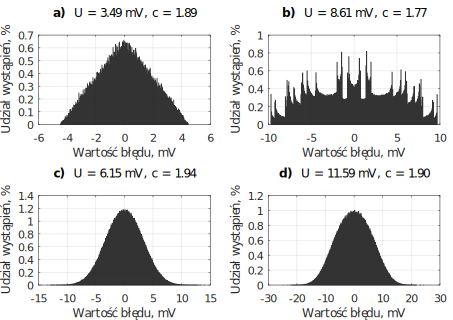
\includegraphics{obrazki/hist_part_a}
\caption{Histogramy błędów \textbf{a)}~statycznego, \textbf{b)}~dynamicznego, \textbf{c)}~losowego, \textbf{d)}~wypadkowego, wielkości wyjściowej zastosowanego w eksperymencie symulacyjnym przetwornika pomiarowego \label{fig_symul_parta_hist}}
\end{center}
\end{figure}

Wyznaczona na drodze eksperymentu niepewność $U_{a,\Sigma}$ wyniosła \qty{11.72}{mV}, przy czym współczynnik rozszerzenia $c_{a,\Sigma}$ wyniósł $1.93$. Wartość niepewności oszacowana na podstawie równania \eqref{eqn_sym_parta_uncert_value_a} jest zatem około 5\% większa od wartości uzyskanej na drodze eksperymentu, co wynika z niedoskonałości przyjętej metody wyznaczania niepewności wypadkowej \cite{jakubiec_system}. W przypadku wartości oszacowanej na podstawie równania \eqref{eqn_sym_parta_uncert_value_b} rozbieżność jest nieco mniejsza i wynosi około 2\%, co dowodzi że w analizowanym przypadku spełnione zostały założenia związane z centralnym twierdzeniem granicznym, a przyjęte uproszczenia okazały się nie mieć znaczącego wpływu na wynik obliczeń. Podobna sytuacja ma miejsce w przypadku oszacowanej wartości współczynnika rozszerzenia. Uzyskana wartość wypadkowa wariancji błędu wielkości wyjściowej wyniosła każdorazowo \qty{37.0}{\micro V}, co pokrywa się z wartością wyznaczoną w równaniu \eqref{eqn_sym_parta_var_sum} oraz tą wyznaczaną w równaniu \eqref{eqn_sym_parta_uncert_value_b}. Wyznaczone w równaniach od \eqref{eqn_sym_parta_uncert_stat} do \eqref{eqn_sym_parta_var_dyn} parametry dla składowych błędu statycznego, dynamicznego i losowego również pokrywają się z tymi wyznaczonymi na drodze przeprowadzonego eksperymentu.

Zaproponowana w pracy \cite{jakubiec_system} metoda wyznaczania niepewności wypadkowej, mimo uwzględniania założeń wynikających z centralnego twierdzenia granicznego, zgodnie z uwagami zawartymi w jej opisie, zapewnia wyniki zawyżone o kilka procent w stosunku do wartości uzyskiwanych symulacyjne. Jako, że omawiane rozbieżności są niewielkie oraz ich znak jest dodatni, uzyskiwane wyniki można uznać za prawidłowe. Wadą przedstawionej metody jest jednak konieczność wyznaczania współczynników koherencji, których wartości zależą zarówno od kształtu splatanych rozkładów, jak i od ich wariancji. Wada ta powoduje, że dla rozkładów o niestandardowym kształcie jej obszar zastosowań staje się ograniczony. Jak wykazały przeprowadzone eksperymenty i obliczenia, splatając kilka rozkładów cechujących się wartością niepewności rozszerzonej tego samego rzędu, obliczenia można uprościć zakładając kształt rozkładu wynikowego zbliżony do kształtu rozkładu normalnego.

Wobec przedstawionych rozważań i przeprowadzonego eksperymentu można stwierdzić, że zaproponowany model błędu odpowiednio opisuje związki pomiędzy kolejnymi błędami, zachodzące w analizowanym obiekcie. Z punktu widzenia analizy całości toru pomiarowego przeprowadzony proces wyznaczania parametrów wypadkowych w przypadku grupy błędów dynamicznych oraz wyznaczanie parametrów wypadkowego błędu wielkości wyjściowej był bezzasadny i został przeprowadzony jedynie w celu weryfikacji zaproponowanej metody obliczeń. Jako, że kolejne fragmenty toro pomiarowego posiadają nieidealne właściwości dynamiczne, będą one wpływać na widmo sygnału wyjściowego błędu dynamicznego analizowanego fragmentu toru pomiarowego. W przypadku pozostałych grup błędów wyznaczenie ich parametrów wypadkowych pozwoli uprościć dalszą analizę ze względu na fakt, że cechują się one typowymi kształtami rozkładów -- w innym przypadku dalsze wyznaczanie wartości współczynników koherencji byłoby problematyczne, co pokazano w omówionym przykładzie.

\begin{comment}
\section{Analiza wzmacniacza pomiarowego}



\section{Analiza przetwornika analogowo-cyfrowego}



\section{Analiza algorytmu transformacji falkowej}


\section{Podsumowanie przeprowadzonego eksperymentu}



\end{comment}
